\documentclass[]{article}
\usepackage[margin=0.25in]{geometry}
\usepackage{pgfplots}
\pgfplotsset{width=10cm,compat=1.9}

\author{Sabrina}

\begin{document}
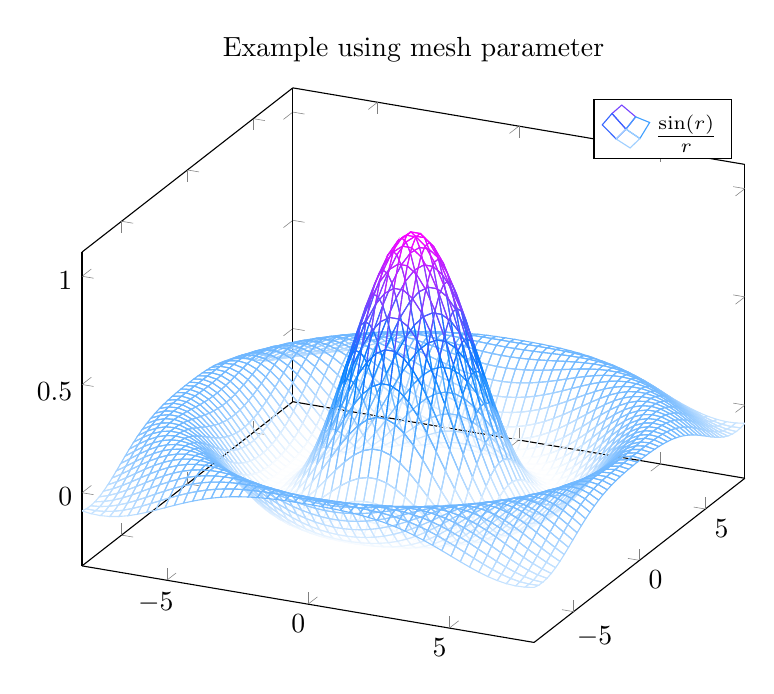
\begin{tikzpicture}
 \begin{axis}[title={Example using mesh parameter}, colormap/cool]
    \addplot3[mesh, samples=50,  domain=-8:8, y domain=-8:8] 
    {sin(deg(sqrt(x^2 + y^2)))/sqrt(x^2 + y^2)};
    \addlegendentry{\(\frac{\sin(r)}{r}\)}
 \end{axis}
\end{tikzpicture}
\begin{tikzpicture}
\begin{axis}
[
    title={Contour plot, view from top},
    view={0}{90}
]
\addplot3[
    contour gnuplot={levels={0.8, 0.4, 0.2, -0.2}}
]
{sin(deg(sqrt(x^2+y^2)))/sqrt(x^2+y^2)};
\end{axis}
\end{tikzpicture}

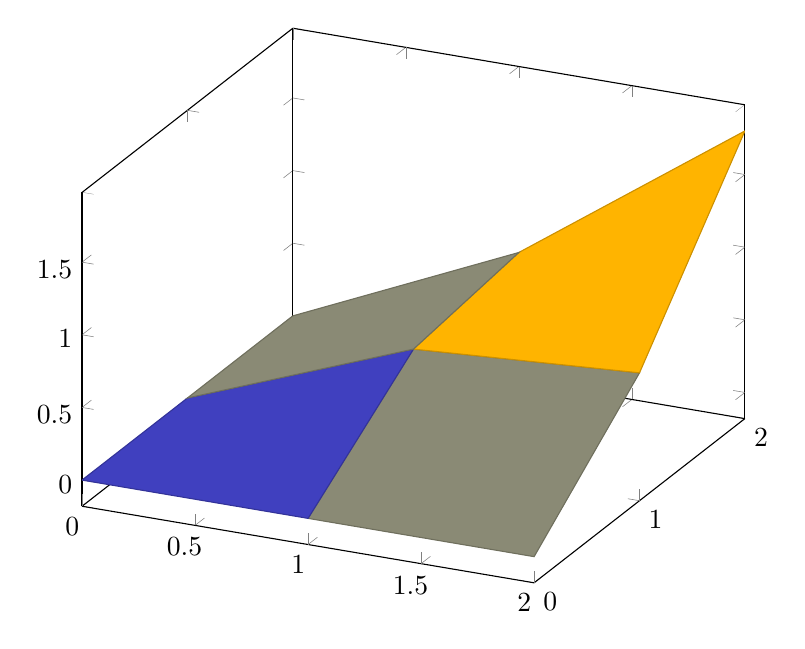
\begin{tikzpicture}
\begin{axis}
\addplot3[
surf,
]coordinates {
(0,0,0) (0,1,0) (0,2,0)

(1,0,0) (1,1,0.6) (1,2,0.7)

(2,0,0) (2,1,0.7) (2,2,1.8)
};
\end{axis}
\end{tikzpicture}

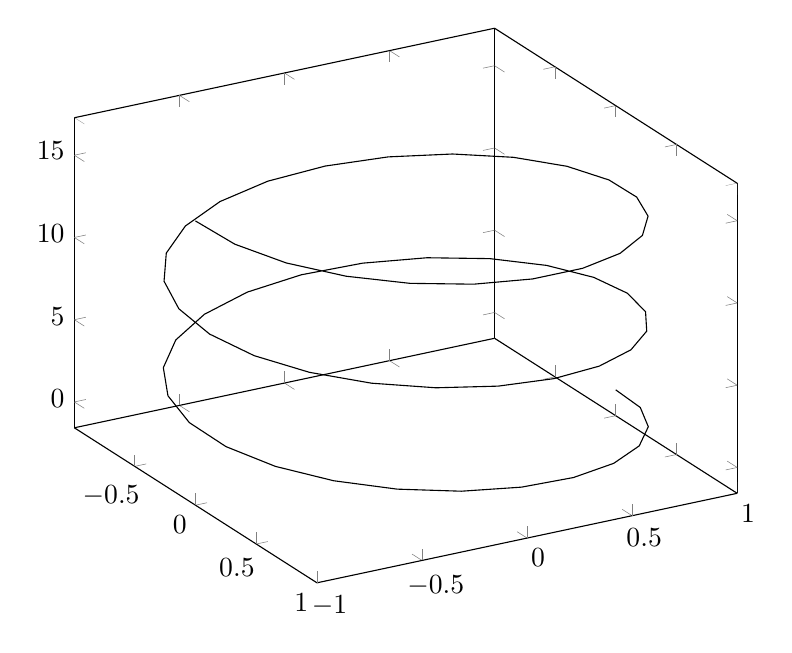
\begin{tikzpicture}
\begin{axis}
    [
    view={60}{30},
    ]
\addplot3[
    domain=0:5*pi,
    samples = 60,
    samples y=0,
]
({sin(deg(x))},
{cos(deg(x))},
{x});
\end{axis}
\end{tikzpicture}
\end{document}

